\documentclass[11pt, a4paper]{article}

% ─── Core Packages ──────────────────────────────────────────────────────────
\usepackage[T1]{fontenc}
\usepackage[utf8]{inputenc}
\usepackage[margin=0.95in, top=1in, bottom=1in]{geometry}
\usepackage{xcolor}
\usepackage{titlesec}
\usepackage{enumitem}
\usepackage{booktabs}
\usepackage{array}
\usepackage{tabularx}
\usepackage{tcolorbox}
\tcbuselibrary{breakable, skins, listings}
\usepackage{hyperref}
\usepackage{parskip}
\usepackage{microtype}
\usepackage{setspace}
\usepackage{fancyhdr}
\usepackage{tikz}
\usetikzlibrary{shapes.geometric, arrows.meta, positioning, fit, backgrounds, calc}
\usepackage{amsmath}
\usepackage{amssymb}
\usepackage{multicol}
\usepackage{colortbl}

% ─── Colour Palette ─────────────────────────────────────────────────────────
\definecolor{primarydark}{HTML}{0D1B2A}    % deep navy-black
\definecolor{primary}{HTML}{1B2A4A}        % navy
\definecolor{accent}{HTML}{D64045}         % engineering red
\definecolor{accentblue}{HTML}{2176AE}     % strong blue
\definecolor{accentgreen}{HTML}{2E8B57}    % system green
\definecolor{accentamber}{HTML}{E07B39}    % amber / warning
\definecolor{subtle}{HTML}{4E5D6C}         % slate
\definecolor{lightbg}{HTML}{F2F5F9}        % near-white
\definecolor{darkline}{HTML}{CBD5E0}       % rule grey
\definecolor{greenlight}{HTML}{EAF7EE}
\definecolor{bluelight}{HTML}{E8F2FB}
\definecolor{redlight}{HTML}{FDECEA}
\definecolor{amberlight}{HTML}{FEF3E8}

% ─── Hyperref ───────────────────────────────────────────────────────────────
\hypersetup{
  colorlinks=true, linkcolor=accentblue,
  urlcolor=accentblue,
  pdftitle={ARAIS Product and System Design Overview},
  pdfauthor={AI/ML Systems Architecture}
}

% ─── Header / Footer ────────────────────────────────────────────────────────
\pagestyle{fancy}\fancyhf{}
\renewcommand{\headrulewidth}{0pt}
\fancyhead[L]{%
  
\begin{tikzpicture}[remember picture, overlay]
    \fill[primary] (0,0) rectangle (\paperwidth, 0.45cm);
  \end{tikzpicture}%
  \hspace{-0.95in}\textcolor{white}{\footnotesize\bfseries\quad ARAIS — Product \& System Design Overview \hfill AI/ML Systems Architecture\quad}%
}
\fancyfoot[C]{\small\color{subtle}--- \thepage\ ---}
\setlength{\headheight}{20pt}
\setlength{\footskip}{20pt}

% ─── Layout Tuning ─────────────────────────────────────────────────────────
\raggedbottom
\setstretch{1.05}
\setlength{\columnsep}{18pt}
\setlength{\tabcolsep}{6pt}
\renewcommand{\arraystretch}{1.25}
\setlist{topsep=4pt, itemsep=3pt, parsep=0pt, partopsep=0pt}

% ─── Section Styling ────────────────────────────────────────────────────────
\titleformat{\section}{\large\bfseries\color{primary}}
  {}{0em}{\colorbox{primary}{\parbox{\dimexpr\linewidth-2\fboxsep\relax}
  {\textcolor{white}{\thesection\quad #1}}}}
\titleformat{\subsection}{\normalsize\bfseries\color{primary}}
  {\color{accent}\thesubsection.}{0.5em}{}[{\color{accent}\titlerule[0.5pt]}]
\titleformat{\subsubsection}{\small\bfseries\color{subtle}}
  {}{0em}{}
\titlespacing{\section}{0pt}{16pt}{8pt}
\titlespacing{\subsection}{0pt}{12pt}{5pt}
\titlespacing{\subsubsection}{0pt}{8pt}{3pt}

% ─── Custom Boxes ───────────────────────────────────────────────────────────
\tcbset{
  reportbox/.style={
    breakable,
    arc=2pt,
    boxrule=1pt,
    left=7pt,
    right=7pt,
    top=5pt,
    bottom=5pt,
    attach boxed title to top left={yshift=-2mm, xshift=5mm},
    boxed title style={arc=2pt, boxrule=0pt},
    fonttitle=\bfseries
  }
}

\newtcolorbox{infobox}[2][accentblue]{
  reportbox, colback=bluelight, colframe=#1,
  title={\small\bfseries\color{white}\ #2\ },
  boxed title style={colback=#1, arc=2pt, boxrule=0pt}
}
\newtcolorbox{greenbox}[1]{
  reportbox, colback=greenlight, colframe=accentgreen,
  title={\small\bfseries\color{white}\ #1\ },
  boxed title style={colback=accentgreen, arc=2pt, boxrule=0pt}
}
\newtcolorbox{redbox}[1]{
  reportbox, colback=redlight, colframe=accent,
  title={\small\bfseries\color{white}\ #1\ },
  boxed title style={colback=accent, arc=2pt, boxrule=0pt}
}
\newtcolorbox{amberbox}[1]{
  reportbox, colback=amberlight, colframe=accentamber,
  title={\small\bfseries\color{white}\ #1\ },
  boxed title style={colback=accentamber, arc=2pt, boxrule=0pt}
}
\newtcolorbox{darkbox}{
  breakable, colback=primary!8, colframe=primary,
  arc=2pt, boxrule=1pt, left=8pt, right=8pt, top=6pt, bottom=6pt
}
\newtcolorbox{notebox}{
  breakable, colback=lightbg, colframe=darkline,
  arc=2pt, boxrule=0.6pt, left=7pt, right=7pt, top=5pt, bottom=5pt
}

% ─── Utility commands ───────────────────────────────────────────────────────
\newcommand{\clabel}[2]{%
  \textcolor{white}{\colorbox{#1}{\footnotesize\bfseries\,#2\,}}%
}
\newcommand{\decision}[1]{\textbf{\textcolor{accentblue}{#1}}}
\newcommand{\component}[1]{\textbf{\textcolor{primary}{#1}}}
\newcommand{\notrecommended}{\clabel{accent}{NOT RECOMMENDED}}
\newcommand{\recommended}{\clabel{accentgreen}{RECOMMENDED}}
\newcommand{\neutral}{\clabel{subtle}{CONDITIONAL}}

% ════════════════════════════════════════════════════════════════════════════
\begin{document}
% ════════════════════════════════════════════════════════════════════════════

% ─── Cover Block ────────────────────────────────────────────────────────────
\thispagestyle{empty}
\begin{tikzpicture}[remember picture, overlay]
  \fill[primarydark] (current page.north west) rectangle
    ([yshift=-7.2cm]current page.north east);
  \fill[accent] ([yshift=-7.2cm]current page.north west) rectangle
    ([yshift=-7.7cm]current page.north east);
\end{tikzpicture}

\vspace*{1.6cm}
\begin{center}
  \begin{minipage}{0.94\linewidth}
    \centering
    {\fontsize{9}{11}\selectfont\color{darkline}\bfseries\MakeUppercase{Product \&\ System Design Overview}}\\[8pt]
    {\fontsize{22}{27}\selectfont\bfseries\color{white}
      Adaptive Real-World\\[4pt]Anomaly Intelligence System}\\[6pt]
    {\fontsize{13}{16}\selectfont\color{accent!70!white}\bfseries ARAIS}\\[16pt]
    {\small\color{darkline}
      Gaps Addressed:\quad
      \colorbox{accent!80!black}{\textcolor{white}{\small\bfseries Gap 1: Evaluation}}\;
      \colorbox{accentblue!90!black}{\textcolor{white}{\small\bfseries Gap 2: Adaptability}}\;
      \colorbox{accentamber!90!black}{\textcolor{white}{\small\bfseries Gap 6: Open-World}}
    }\\[18pt]
    {\small\color{subtle} AI/ML Systems Architecture \textbf{·} April 2026}
  \end{minipage}
\end{center}
\vfill

\begin{darkbox}
\noindent\textbf{\color{primary}Document Purpose.}\quad
This document defines the product form, interaction model, system behaviour,
learning strategy, component architecture, and technology direction for ARAIS.
It is a \textit{design brief} — not an implementation specification.
Every decision herein is justified against three constraints: local compute only,
no paid cloud services, and the need to demonstrate production-grade intelligence
within a single-developer or small-team build.
\end{darkbox}

\newpage

% ─── Table of Contents strip ────────────────────────────────────────────────
\begin{tcolorbox}[enhanced, colback=primary, colframe=primary, arc=2pt,
  left=8pt, right=8pt, top=6pt, bottom=6pt, boxsep=1.5pt]
  \color{white}\bfseries\small
  \begin{multicols}{2}
  \raggedright
  1.\quad Product Form \& Architecture Decision\\
  2.\quad Core User Interaction Model\\
  3.\quad System Behaviour (High-Level)\\
  4.\quad Learning Strategy\\
  5.\quad System Components\\
  6.\quad Technology Direction\\
  7.\quad Scope Boundaries\\
  \columnbreak
  \normalfont\color{darkline}\small
  \textit{Architecture justification, desktop-first rationale}\\
  \textit{Inputs, outputs, data types, interaction modes}\\
  \textit{Data flow, adaptive switching, OOD handling}\\
  \textit{Pre-trained, incremental, resource-aware}\\
  \textit{Seven major blocks and their responsibilities}\\
  \textit{MERN, Electron, Python IPC, local databases}\\
  \textit{What ARAIS explicitly does not attempt}
  \end{multicols}
\end{tcolorbox}

\vspace{6pt}

% ════════════════════════════════════════════════════════════════════════════
\section{Product Form \& Architecture Decision}
% ════════════════════════════════════════════════════════════════════════════

\subsection{What Are We Building?}

ARAIS is a \textbf{local-first, desktop-grade intelligent anomaly detection workbench}.
It runs entirely on a user's machine, accepts time-series and structured data,
runs multiple anomaly detection models under a shared adaptive orchestration layer,
and surfaces results through a rich dashboard interface — all without requiring
internet access or a paid cloud backend.

This is not a cloud SaaS product and not a pure CLI research tool.
It is positioned as a \textit{developer and analyst workbench} — something between
a Jupyter notebook and a production monitoring tool, designed to demonstrate
serious system-level intelligence within constrained infrastructure.

\vspace{6pt}
\subsection{Architecture Decision: Why Not Pure Web (MERN)?}

\begin{infobox}{Architecture Evaluation: MERN Stack}
A standard MERN (MongoDB, Express, React, Node) stack assumes a persistent server
process, a browser client, and a clear request/response boundary.
For ARAIS, this creates three structural mismatches:

\begin{enumerate}[leftmargin=1.2em, itemsep=3pt]
  \item \textbf{ML compute lives in Python.} Node.js has no credible native ML runtime.
  Every model inference call must bridge to Python — which MERN has no clean
  mechanism for without a separate service layer, adding latency and deployment complexity.

  \item \textbf{No server to host.} Without paid cloud, a ``server'' means a locally-running
  Express process the user must manually start. This degrades UX significantly
  and adds operational friction for a local tool.

  \item \textbf{Browser sandboxing limits filesystem access.} File uploads, 
  local model checkpoints, and SQLite/MongoDB data paths all require server
  mediation in a web context — an unnecessary indirection for a local system.
\end{enumerate}

\noindent\notrecommended\quad as the \textit{primary} architecture.
MERN's React layer is valuable; its server model is not appropriate here.
\end{infobox}

\vspace{6pt}
\subsection{Final Recommended Architecture}

\begin{greenbox}{Recommended: Electron + React (UI) + Python Backend (ML Engine)}
\textbf{Electron} provides a desktop shell that embeds a Chromium renderer 
(for the React UI) and a Node.js main process (for filesystem, IPC, and database access),
without requiring a separate server process.
The user launches one executable; everything runs locally.

\textbf{Python ML Engine} runs as a managed child process,
spawned and supervised by Electron's main process.
Communication happens over a lightweight local HTTP interface (FastAPI on localhost)
or stdin/stdout IPC — both zero-infrastructure, zero-latency, no external dependency.

\textbf{React dashboard} (within Electron) provides the full UI:
data upload, stream visualisation, anomaly results, evaluation reports,
and model control panels. It communicates with the Python engine through
Electron's IPC bridge or the local FastAPI endpoint.

\medskip
\noindent The result is a \textbf{single installable application} with:
no server management, no browser security restrictions, full filesystem access,
full Python ML capability, and a production-grade React interface.
\end{greenbox}

\vspace{6pt}
\begin{notebox}
\noindent\textbf{Why not pure Python + Flask?}\quad
Flask/Django + Jinja templates produce UIs that look and behave like 2015-era web apps.
ARAIS requires real-time streaming visualisations, live confidence gauges, and interactive
model control — capabilities that belong in React, not server-rendered HTML.
The Electron bridge gives us both without compromise.
\end{notebox}

\vspace{4pt}
\begin{center}
\begin{tikzpicture}[node distance=0.6cm and 1.0cm,
  box/.style={rectangle, rounded corners=3pt, minimum width=2.8cm, minimum height=0.85cm,
    text centered, font=\small\bfseries},
  arr/.style={-Stealth, thick, color=subtle}]

  \node[box, fill=primary, text=white] (ui) {React UI\\(Electron Renderer)};
  \node[box, fill=accentblue!20, text=primary, right=1.4cm of ui] (ipc) {Electron Main\\+ IPC Bridge};
  \node[box, fill=accentgreen!20, text=primary, right=1.4cm of ipc] (py) {Python ML Engine\\(FastAPI)};
  \node[box, fill=subtle!15, text=primary, below=0.6cm of ipc] (db) {Local DB\\(SQLite / MongoDB)};

  \draw[arr] (ui) -- (ipc) node[midway, above, font=\tiny\color{subtle}]{events};
  \draw[arr] (ipc) -- (py) node[midway, above, font=\tiny\color{subtle}]{HTTP/IPC};
  \draw[arr] (py) -- (ipc) node[midway, below, font=\tiny\color{subtle}]{results};
  \draw[arr] (ipc) -- (ui) node[midway, below, font=\tiny\color{subtle}]{state update};
  \draw[arr] (ipc) -- (db);
  \draw[arr] (py) -- (db);
\end{tikzpicture}
\end{center}

% ════════════════════════════════════════════════════════════════════════════
\section{Core User Interaction Model}
% ════════════════════════════════════════════════════════════════════════════

\subsection{Inputs: What the System Accepts}

ARAIS accepts three categories of input, each targeting a distinct usage scenario:

\vspace{4pt}
\begin{tabularx}{\linewidth}{>{\bfseries\color{primary}}p{3.2cm} X >{\small\color{subtle}}p{3.4cm}}
\toprule
\rowcolor{primary!8}
\color{primary}Input Type & \color{primary}Description & \color{primary}Typical Source\\
\midrule
Time-series files & Univariate or multivariate sequences: CPU metrics, sensor readings, log-derived numeric streams & System telemetry exports, IoT logs\\
\addlinespace[2pt]
CSV / JSON upload & Tabular structured data with a timestamp column and one or more value columns & Analytics exports, database dumps\\
\addlinespace[2pt]
Simulated stream & Internally generated real-time signal with configurable noise, drift, and anomaly injection rate & Built-in simulation engine\\
\bottomrule
\end{tabularx}

\vspace{8pt}
\textbf{How users provide data} — three interaction modes are supported:

\begin{enumerate}[leftmargin=1.5em, itemsep=4pt]
  \item \textbf{File upload via UI drag-and-drop.} The most common path.
  Users drag CSV/JSON files onto the dashboard; the system parses and indexes them locally.

  \item \textbf{Local API endpoint (FastAPI).} For programmatic ingestion.
  A local REST endpoint accepts POST requests with structured payloads,
  enabling integration with scripts, data pipelines, or scheduled jobs
  running on the same machine.

  \item \textbf{Simulated real-time stream.} The built-in stream simulator
  generates time-series data at configurable rates, injecting Gaussian noise,
  step-change drift, and labelled anomaly events.
  This mode is critical for demonstrating Gap 1 (evaluation under realistic conditions)
  without requiring live external data.
\end{enumerate}

\subsection{Outputs: What the System Returns}

Every inference pass through ARAIS produces a structured output bundle,
not a single binary label. The output surface is designed around the principle
that \textit{every prediction should communicate what the model knows,
what it doesn't know, and how confident it is in that distinction.}

\vspace{4pt}
\begin{tabularx}{\linewidth}{>{\bfseries\color{primary}}p{4.2cm} X}
\toprule
\rowcolor{primary!8}
\color{primary}Output & \color{primary}Meaning\\
\midrule
Anomaly flag & Binary label: \texttt{NORMAL} / \texttt{ANOMALY}, per data point or window\\
\addlinespace[2pt]
Risk score & Continuous score $[0, 1]$ quantifying anomaly severity\\
\addlinespace[2pt]
Model confidence & Softmax or calibrated probability assigned by the active detector\\
\addlinespace[2pt]
Epistemic uncertainty & Model-level uncertainty (high = model is unsure about this region)\\
\addlinespace[2pt]
OOD proximity flag & Distance from training distribution; triggers novel-anomaly alert\\
\addlinespace[2pt]
Novel anomaly alert & Structured alert when input is detected as out-of-distribution\\
\addlinespace[2pt]
Evaluation report & Per-session performance profile: accuracy under noise/drift levels,
  latency histogram, model switch log\\
\bottomrule
\end{tabularx}

\vspace{6pt}
\begin{amberbox}{Key Design Principle: Outputs Drive Action}
ARAIS does not just report anomalies — it communicates the \textit{quality} of its own 
predictions. A high-confidence normal result means something different from a 
low-confidence normal result. An OOD flag means: ``this is anomalous and unlike
anything I was trained on — do not trust my classification.''
These distinctions are first-class outputs, not footnotes.
\end{amberbox}

% ════════════════════════════════════════════════════════════════════════════
\section{System Behaviour (High-Level)}
% ════════════════════════════════════════════════════════════════════════════

\subsection{Data Flow Through the System}

Data moves through ARAIS in a single directed pipeline with three branching decision points:

\vspace{6pt}
\begin{center}
\begin{tikzpicture}[node distance=0.45cm and 0.8cm,
  stage/.style={rectangle, rounded corners=3pt, minimum width=3.0cm, minimum height=0.8cm,
    text centered, font=\small\bfseries, text width=3.0cm},
  decision/.style={diamond, aspect=2.2, minimum width=2.8cm, minimum height=0.75cm,
    text centered, font=\scriptsize\bfseries, text width=2.4cm, inner sep=1pt},
  arr/.style={-Stealth, thick, color=subtle},
  lbl/.style={font=\tiny\color{subtle}, midway}]

  \node[stage, fill=accentblue!20, text=primary] (ingest) {1. Data Ingestion\\Layer};
  \node[stage, fill=primary!10, text=primary, below=0.55cm of ingest] (preprocess) {2. Preprocessing\\Pipeline};
  \node[decision, fill=accentamber!30, text=primary, below=0.55cm of preprocess] (ood) {OOD\\Check};
  \node[stage, fill=accentgreen!20, text=primary, below=0.55cm of ood] (orchestrate) {3. Adaptive\\Orchestrator};
  \node[stage, fill=primary!15, text=primary, below=0.55cm of orchestrate] (model) {4. Model\\Inference};
  \node[stage, fill=accent!15, text=primary, below=0.55cm of model] (eval) {5. Evaluation\\Engine};
  \node[stage, fill=accentblue!15, text=primary, below=0.55cm of eval] (ui) {6. UI / Output\\Layer};

  % OOD branch
  \node[stage, fill=accent!25, text=primary, right=2.0cm of ood, minimum width=2.6cm] (novel) {Novel Anomaly\\Triage};

  \draw[arr] (ingest) -- (preprocess);
  \draw[arr] (preprocess) -- (ood);
  \draw[arr] (ood) -- (orchestrate) node[lbl, right]{\textit{in-dist.}};
  \draw[arr] (ood) -- (novel) node[lbl, above]{\textit{OOD}};
  \draw[arr] (novel) |- (eval);
  \draw[arr] (orchestrate) -- (model);
  \draw[arr] (model) -- (eval);
  \draw[arr] (eval) -- (ui);
\end{tikzpicture}
\end{center}

\vspace{6pt}
Each stage is described below in behavioural terms:

\begin{enumerate}[leftmargin=1.5em, itemsep=5pt]
  \item \textbf{Ingestion:} Raw data enters through file upload, API call, or the stream simulator.
  The ingestion layer normalises formats, validates schema, and emits a timestamped
  window buffer to the preprocessing pipeline.

  \item \textbf{Preprocessing:} Applies windowing, normalisation, and optional
  noise/drift injection (in evaluation mode). This is also where the
  input statistics (mean, variance, distribution shape) are computed 
  and compared against stored training-time reference statistics —
  the first signal feeding the OOD check.

  \item \textbf{OOD Check:} A lightweight distribution proximity test runs
  \textit{before} model inference. Inputs that fall beyond a configurable
  Mahalanobis distance threshold (or equivalent density-based threshold)
  are routed to the Novel Anomaly Triage path rather than the standard model pool.
  This prevents silent misclassification of genuinely novel events.

  \item \textbf{Adaptive Orchestration:} For in-distribution inputs,
  the orchestrator selects the active model from the pool based on runtime state
  (current latency, system CPU/memory load, declared risk tier of the current session).
  This is the core mechanism addressing Gap 2.

  \item \textbf{Model Inference:} The selected model runs inference and returns
  the anomaly prediction along with its confidence score and uncertainty estimate.

  \item \textbf{Evaluation Engine:} Every inference result is logged and assessed
  against the continuously-updated performance profile. This closes the evaluation loop:
  model performance is measured in real-time against actual input conditions, not
  only on a pre-defined test set.

  \item \textbf{UI / Output:} Results surface in the dashboard as live charts,
  alert panels, confidence gauges, and downloadable evaluation reports.
\end{enumerate}

\subsection{Adaptive Model Switching}

The orchestrator maintains a \textit{runtime state vector} consisting of:
current inference latency (moving average), system CPU utilisation,
session risk tier (set by the user: \texttt{LOW} / \texttt{MEDIUM} / \texttt{HIGH}),
and the recent false-positive rate from the evaluation engine's live monitoring.

Model selection uses a priority rule:
if latency budget is exceeded or CPU load is above threshold, downgrade to
a lighter model regardless of accuracy preference.
If risk tier is \texttt{HIGH} and resources are available, upgrade to the
highest-accuracy available model.
Between these poles, the orchestrator operates on the stored cost-accuracy
frontier profile — a lookup table populated during the offline evaluation phase.

\subsection{Unknown Anomaly Identification}

Novel anomaly handling is three-step:
\textbf{(a)} distribution distance triggers OOD routing before inference;
\textbf{(b)} if inference still runs (e.g., marginal OOD score), high epistemic uncertainty
flags the result as ``uncertain anomaly'' rather than a definitive classification;
\textbf{(c)} all OOD and high-uncertainty events are logged to a
\textit{novel event queue} — a structured buffer that can be reviewed by the user
and optionally added to the retraining dataset. This is the active-learning entry point.

% ════════════════════════════════════════════════════════════════════════════
\section{Learning Strategy}
% ════════════════════════════════════════════════════════════════════════════

\begin{infobox}{Learning Strategy Summary}
ARAIS adopts a \textbf{hybrid learning posture}: pre-trained models as the baseline,
local incremental fine-tuning as the adaptation mechanism,
synthetic data as the primary training substrate for evaluation stress-testing.
No GPU farm. No cloud training API. No downloading multi-gigabyte checkpoints.
\end{infobox}

\vspace{6pt}
\subsubsection{Pre-trained Models (Primary Baseline)}
The system ships with lightweight pre-trained anomaly detectors trained on
publicly available time-series benchmarks (e.g., NAB, KPI-Anomaly, SMD).
These models are small by design — they fit in CPU RAM, load in under two seconds,
and produce usable results out of the box. The user does not need to train anything
to get started. This lowers the barrier to the first meaningful result.

\subsubsection{Local Incremental Training}
When the user uploads domain-specific data, the system supports
\textit{incremental fine-tuning}: adapting the pre-trained model's later layers
(or its normalisation statistics, in the case of reconstruction-based models)
to the new data distribution. This is intentionally shallow — no full retraining,
no multi-hour compute jobs. The goal is distribution adaptation, not architecture search.

\subsubsection{Synthetic Data for Evaluation}
The built-in stream simulator generates synthetic time-series with configurable
anomaly injection, noise schedules, and concept drift rates.
This synthetic data is the \textit{primary vehicle for stress-testing} models
against Gap 1 conditions, entirely locally.
It also serves as augmentation data for incremental training when labelled real data is scarce.

\subsubsection{Lightweight vs.\ Heavy Model Tiering}

\begin{tabularx}{\linewidth}{>{\bfseries\color{primary}}p{3.0cm}
  >{\small}p{3.4cm} >{\small}p{3.4cm} >{\small}X}
\toprule
\rowcolor{primary!8}
\color{primary}Tier & \color{primary}Model Type & \color{primary}Latency Profile & \color{primary}When Used\\
\midrule
Fast (Tier 1) & Statistical (Z-score, EWMA, MAD) & $<$5ms per window & High load, low-risk\\
\addlinespace[2pt]
Medium (Tier 2) & Isolation Forest, LOF, shallow LSTM & 5--50ms & Default operating mode\\
\addlinespace[2pt]
Deep (Tier 3) & Autoencoder, Transformer-lite, DeepSVDD & 50--300ms & Low load, high-risk sessions\\
\bottomrule
\end{tabularx}

% ════════════════════════════════════════════════════════════════════════════
\section{System Components (High-Level)}
% ════════════════════════════════════════════════════════════════════════════

\subsection{Component Map}

Seven major components form the ARAIS operational architecture.
Each is described by \textit{what it does}, not how it is implemented.

\vspace{6pt}

\begin{greenbox}{Component 1 — Data Ingestion Layer}
\textbf{Responsibility:} Accept, validate, and normalise all incoming data regardless of source
(file upload, API call, or internal simulator).
Performs schema validation, timestamp parsing, missing-value flagging,
and format unification into a canonical internal representation
(timestamped floating-point window arrays).

\textbf{Also owns:} The stream simulator engine, which generates configurable synthetic 
time-series for evaluation and demonstration purposes.
\end{greenbox}

\vspace{6pt}

\begin{infobox}{Component 2 — Processing Pipeline}
\textbf{Responsibility:} Transform normalised input into model-ready feature windows.
Applies sliding-window segmentation, z-score normalisation, 
optional lag/difference features, and in evaluation mode,
injects configured noise and drift perturbations.

\textbf{Also owns:} Runtime input statistics (mean, covariance, distribution shape estimates)
that feed the OOD detection module downstream.
\end{infobox}

\vspace{6pt}

\begin{redbox}{Component 3 — Model Layer (Multi-model Pool)}
\textbf{Responsibility:} Host and serve the tiered model pool (Tier 1/2/3 as defined above).
Each model exposes a uniform inference interface:
receive a feature window, return an anomaly score, confidence value,
and uncertainty estimate. Models are loaded lazily and cached in memory.

\textbf{Key property:} No model in the pool is aware of the others.
Composition and switching are entirely the orchestrator's responsibility —
models are stateless inference units.
\end{redbox}

\vspace{6pt}

\begin{amberbox}{Component 4 — Adaptive Decision Engine (Orchestrator)}
\textbf{Responsibility:} The cognitive centre of the system.
Monitors the runtime state vector (latency, load, risk tier, live FP rate)
and selects the active model from the pool for each inference request.

\textbf{Behaviour:} Maintains a cost-accuracy frontier profile per model,
updated continuously from evaluation engine feedback.
Issues model-switch events when runtime conditions cross defined thresholds.
Logs every switch decision with its triggering reason — providing
full auditability of adaptive behaviour.
\end{amberbox}

\vspace{6pt}

\begin{redbox}{Component 5 — Open-World Detection Module}
\textbf{Responsibility:} Intercept inputs that fall outside the known distribution
\textit{before} they reach the model layer, and handle high-uncertainty
model outputs with appropriate escalation.

\textbf{Two-layer defence:}
(a) Pre-inference OOD screen using distribution distance metrics applied
to the processing pipeline's runtime statistics;
(b) Post-inference uncertainty threshold check, flagging results where
epistemic uncertainty exceeds a calibrated bound.
All flagged events are routed to the novel event queue.
\end{redbox}

\vspace{6pt}

\begin{infobox}[accentgreen]{Component 6 — Evaluation Engine}
\textbf{Responsibility:} Continuous, live model assessment — not a batch report run post-hoc.
Records every inference result alongside input conditions (noise estimate,
drift rate, input distribution distance from baseline).
Builds and updates a per-model performance profile: precision, recall,
false-positive rate, latency percentiles, all segmented by condition.

\textbf{Key output:} The evaluation report surfaced to the user is generated from
this live profile — not from a static holdout run.
This directly addresses Gap 1.
\end{infobox}

\vspace{6pt}

\begin{infobox}{Component 7 — UI / Dashboard Layer}
\textbf{Responsibility:} Present all system outputs in a clear, interactive interface.
Four primary panels: (1) Live stream visualiser with anomaly overlays;
(2) Inference result panel with confidence gauges and uncertainty indicators;
(3) Model status panel showing active model, recent switch events, and cost-accuracy frontier;
(4) Evaluation report viewer with performance profiles under different conditions.

\textbf{Technology:} React within Electron. Communicates with the Python engine
via the Electron IPC bridge. All state is local.
\end{infobox}

% ════════════════════════════════════════════════════════════════════════════
\section{Technology Direction (Free Tools Only)}
% ════════════════════════════════════════════════════════════════════════════

\vspace{4pt}
\begin{tabularx}{\linewidth}{>{\bfseries\color{primary}}p{3.6cm}
  >{\small}p{3.0cm} X}
\toprule
\rowcolor{primary!8}
\color{primary}Technology & \color{primary}Role & \color{primary}Justification\\
\midrule
Electron (v28+) & Desktop shell & Unified app packaging; Node.js main process manages Python subprocess, filesystem, and IPC\\
\addlinespace[3pt]
React (v18+) & UI framework & Component-based real-time dashboards; Recharts/Victory for live stream visualisation\\
\addlinespace[3pt]
Python 3.11+ & ML engine runtime & Ecosystem lock-in for scikit-learn, PyTorch, statsmodels; runs as managed subprocess\\
\addlinespace[3pt]
FastAPI & Internal API layer & Lightweight local HTTP server within the Python engine; typed endpoints, auto-docs\\
\addlinespace[3pt]
scikit-learn & Tier 1/2 models & Isolation Forest, LOF, OCSVM — battle-tested, CPU-native, no GPU required\\
\addlinespace[3pt]
PyTorch (CPU) & Tier 3 models & Autoencoder, lightweight Transformer; CPU inference only; quantised models preferred\\
\addlinespace[3pt]
SQLite & Operational store & Inference log, evaluation records, session history; zero-server, file-based, embedded\\
\addlinespace[3pt]
MongoDB (local) & Dataset storage & Flexible schema for ingested time-series datasets and model metadata\\
\addlinespace[3pt]
ZeroMQ (optional) & Streaming IPC & If stdin/stdout IPC proves insufficient for high-frequency streams; lightweight, no broker\\
\addlinespace[3pt]
NumPy / Pandas & Data processing & Standard time-series manipulation within the processing pipeline\\
\addlinespace[3pt]
River (optional) & Online learning & Incremental/online ML library; natural fit for the adaptive fine-tuning path\\
\bottomrule
\end{tabularx}

\vspace{8pt}
\begin{notebox}
\noindent\textbf{On MERN's place in this stack:}
The ``M'' (MongoDB) and ``R'' (React) from MERN are directly adopted.
The ``E'' (Express) and ``N'' (Node as server) are replaced by
Electron's main process (for IPC and OS integration) and Python/FastAPI
(for ML serving). This hybrid takes the best of MERN's front-end tooling
and discards the server model that does not fit a local-first architecture.
\end{notebox}

% ════════════════════════════════════════════════════════════════════════════
\section{Scope Boundaries — What ARAIS Does Not Build}
% ════════════════════════════════════════════════════════════════════════════

Scope discipline is as important as scope definition.
The following boundaries are deliberate design decisions, not compromises.

\vspace{6pt}
\begin{tabularx}{\linewidth}{>{\bfseries\color{accent}}p{4.8cm} X}
\toprule
\rowcolor{accent!8}
\color{primary}Out of Scope & \color{primary}Reasoning\\
\midrule
Distributed compute / cluster deployment & ARAIS is a single-machine system.
  Distributed infrastructure would obscure the system-design intelligence behind
  DevOps complexity, adding cost with no research contribution.\\
\addlinespace[3pt]
Billion-record / petabyte-scale data & The domain is streaming and batch time-series
  at sensor/log scale. Massive-data infrastructure (Spark, Flink, Kafka clusters)
  is a different problem class entirely.\\
\addlinespace[3pt]
Paid cloud services (AWS, GCP, Azure) & Explicit constraint. No inference APIs,
  no managed databases, no object storage, no deployment pipelines.\\
\addlinespace[3pt]
Custom model architecture research & ARAIS orchestrates and evaluates models;
  it does not design new neural architectures. The model pool uses
  established, well-understood approaches.\\
\addlinespace[3pt]
Production SLA / enterprise hardening & No multi-tenancy, no RBAC, no HA failover.
  This is an intelligence demonstration platform, not a production SaaS.\\
\addlinespace[3pt]
Automated full retraining pipelines & Incremental adaptation is in scope.
  Full retraining (dataset versioning, hyperparameter search, CI/CD for models)
  is explicitly deferred.\\
\bottomrule
\end{tabularx}

\vspace{8pt}
\begin{darkbox}
\noindent\textbf{\color{white}What ARAIS \textit{is} optimised for:}
\begin{itemize}[leftmargin=1.2em, itemsep=3pt]
  \item \textcolor{accentgreen}{\textbf{Simulation of real-world conditions}} —
    noise injection, drift scheduling, OOD event generation, all locally
  \item \textcolor{accentblue}{\textbf{Demonstrable adaptive intelligence}} —
    visible model switching, live cost-accuracy trade-offs, auditability
  \item \textcolor{accentamber}{\textbf{Strong system design}} —
    clean component separation, well-defined interfaces, closed-loop evaluation
  \item \textcolor{accent}{\textbf{Honest uncertainty communication}} —
    every prediction carries confidence and OOD signals, not just a label
\end{itemize}
\end{darkbox}

\vspace{16pt}
\noindent\color{accent}\rule{\linewidth}{1.2pt}
\vspace{6pt}

\begin{center}
{\large\bfseries\color{primary} System Design Summary}
\end{center}

\vspace{4pt}
\begin{tabularx}{\linewidth}{>{\bfseries\color{primary}}p{4.0cm} X}
\toprule
\rowcolor{primary!8}
\color{primary}Dimension & \color{primary}Decision\\
\midrule
Product form & Desktop application (Electron) — local-first, single executable\\
UI technology & React 18 within Electron renderer\\
ML runtime & Python 3.11 + FastAPI, managed subprocess\\
Communication & Electron IPC + local HTTP; ZeroMQ optional for high-frequency\\
Primary database & SQLite (operational) + MongoDB local (dataset storage)\\
Model strategy & Pre-trained baselines + incremental fine-tuning; 3-tier pool\\
Evaluation posture & Continuous live profiling, not batch holdout\\
OOD handling & Pre-inference distribution check + post-inference uncertainty gate\\
Adaptivity mechanism & Runtime state vector $\rightarrow$ orchestrator $\rightarrow$ model switch\\
Scope anchor & Single-machine, demonstration-grade, research-quality design\\
\bottomrule
\end{tabularx}

\vspace{12pt}
\noindent\color{accent}\rule{\linewidth}{1.2pt}
\begin{center}
  \small\color{subtle}
  \textit{ARAIS — Product \& System Design Overview}\\
  \textit{Version 1.0 · AI/ML Systems Architecture · April 2026}\\
  \textit{This document is a design brief for senior engineers, architects, and technical reviewers.}
\end{center}

\end{document}